\section{時間分解能を悪化させる要素の考察}
図\ref{fg:Treso_JittervsGain_Minus} から、35 倍以上で過剰ノイズと考えられる影響が支配的になることで、時間分解能が悪化することを示した。
時間分解能が良い190 Vと悪い198 Vの波形を比較することで、この時間分解能が悪化する要因の考察を進める。

図\ref{fg:waveform_190V} に190 V の波形、図\ref{fg:waveform_198V} に198 V の波形を示す。
この図はオシロスコープの出力で、横軸が時間で縦軸が波高である。
2つの波形を比較すると、198 V の波形は波高に大きなばらつきがあることがわかる。
198 Vの波形を見ると、波高が小さい波形よりも波高が大きい波形の方が、波高が最大の時の時間が遅いことがわかる。
これは、検出器内で生成された電子が電極に向かって進む際に、高電場による電子雪崩によって新たに電子正孔対を発生させる過程が何度も繰り返され、
その過程の回数が多いほど、電子の数が増えることによって信号が大きくなり、その信号が電極に誘起される時間が遅くなるからであると考える。
この過程によって生じる信号由来の波高の揺らぎが、最大波高の50%にばらつき$\sigma_s$を与え、それによって到達時間のばらつきを増加させ、時間分解能が悪化に影響していると考える。

\begin{figure}[h]
    \begin{minipage}[b]{0.5\linewidth}
        \centering
        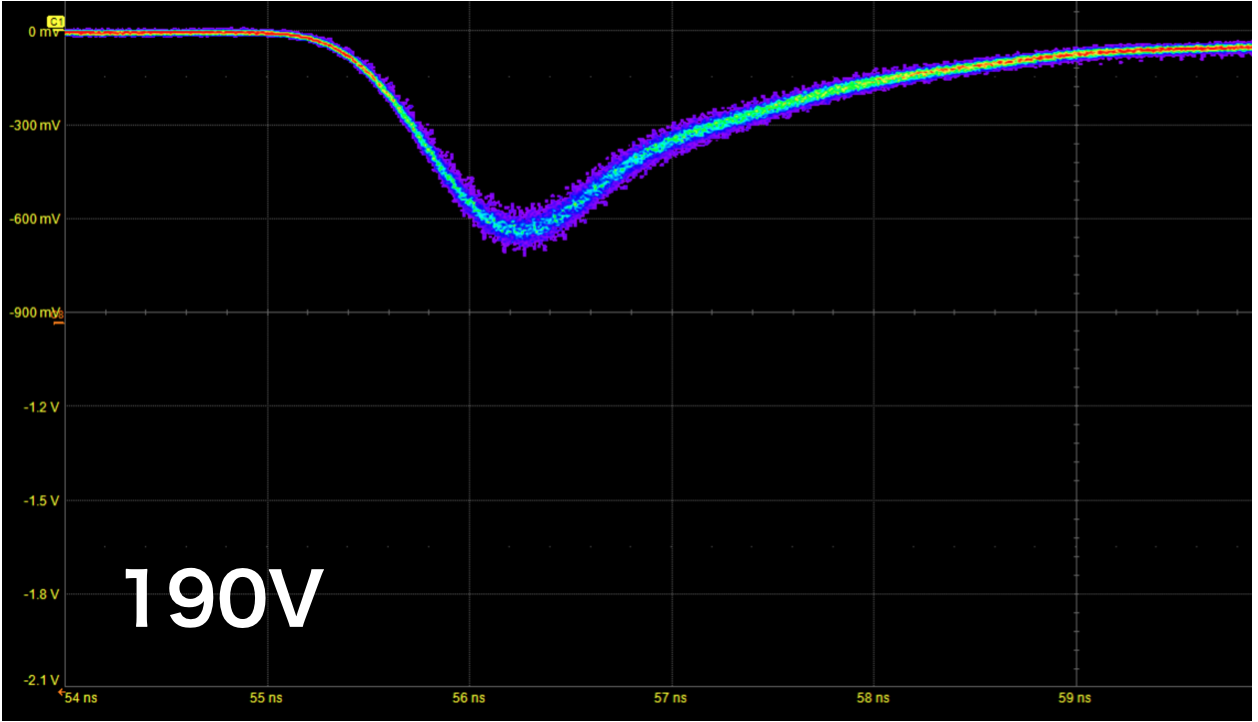
\includegraphics[width=8cm]{fig/ch5/waveform_190V.png}
        \subcaption{190Vの信号の波形}
        \label{fg:waveform_190V}
    \end{minipage}
    \begin{minipage}[b]{0.5\linewidth}
        \centering
        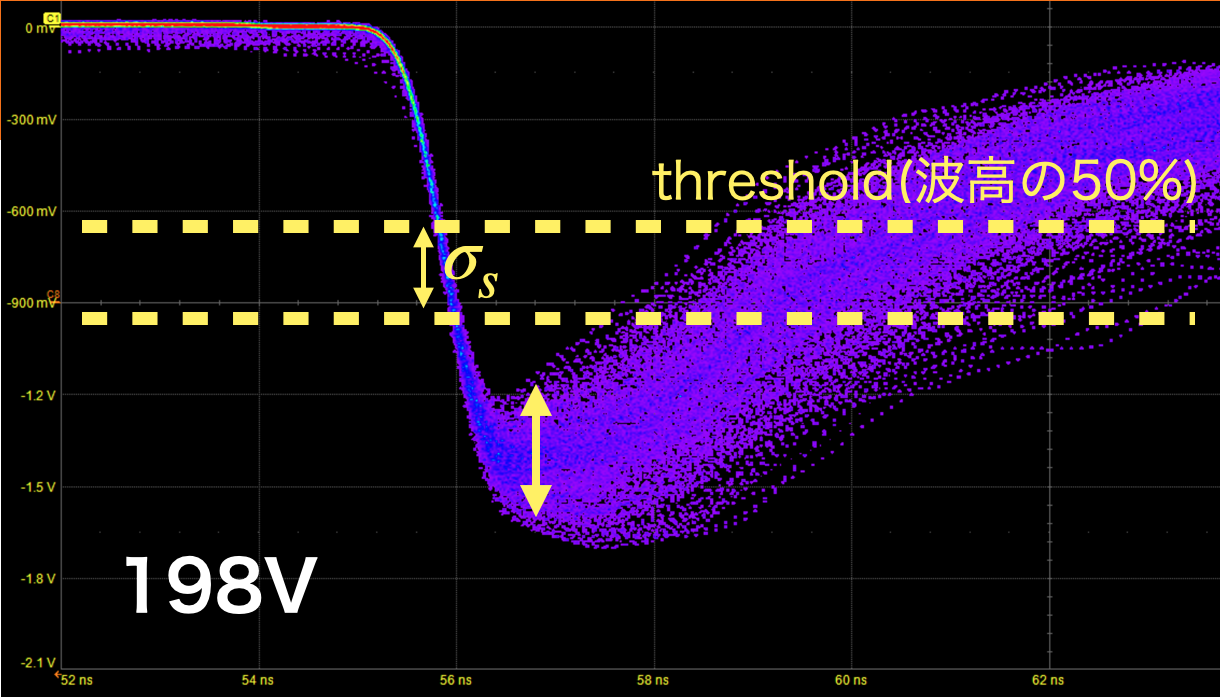
\includegraphics[width=8cm]{fig/ch5/waveform_198V.png}
        \subcaption{198Vの信号の波形}
        \label{fg:waveform_198V}
    \end{minipage}
    \caption[オシロスコープの出力の比較]{オシロスコープの出力の比較\\198 V の波形から波高の揺らぎが大きいことがわかる。そのため、増幅率が増加すると波高の50%のばらつき$\sigma_s$の影響が大きくなる。}
\end{figure}

%波高のばらつきが実際に時間分解能に影響するのかを調べるために、図\ref{fg:APD_2Dhist} に190 V と198 V の時の到達時間と波高の2次元ヒストグラムを示す。
%190 V のヒストグラムからは到達時間のばらつきは少ないが見えないが、198 V のヒストグラムでは、55.5 ns 以下の領域に多くの点があることがわかった。
%この点があることによって到達時間の標準偏差が大きくなってしまうと考える。
%よって、時間分解能を悪化する原因は、電圧を大きくすることによる波高のばらつきの増加によるものであると考える。
%この信号由来の波高のばらつきの影響が、時間分解能にどのくらい関わっているのかを調べた。
%
%\begin{figure}[h]
%    \begin{minipage}[b]{0.5\linewidth}
%        \centering
%        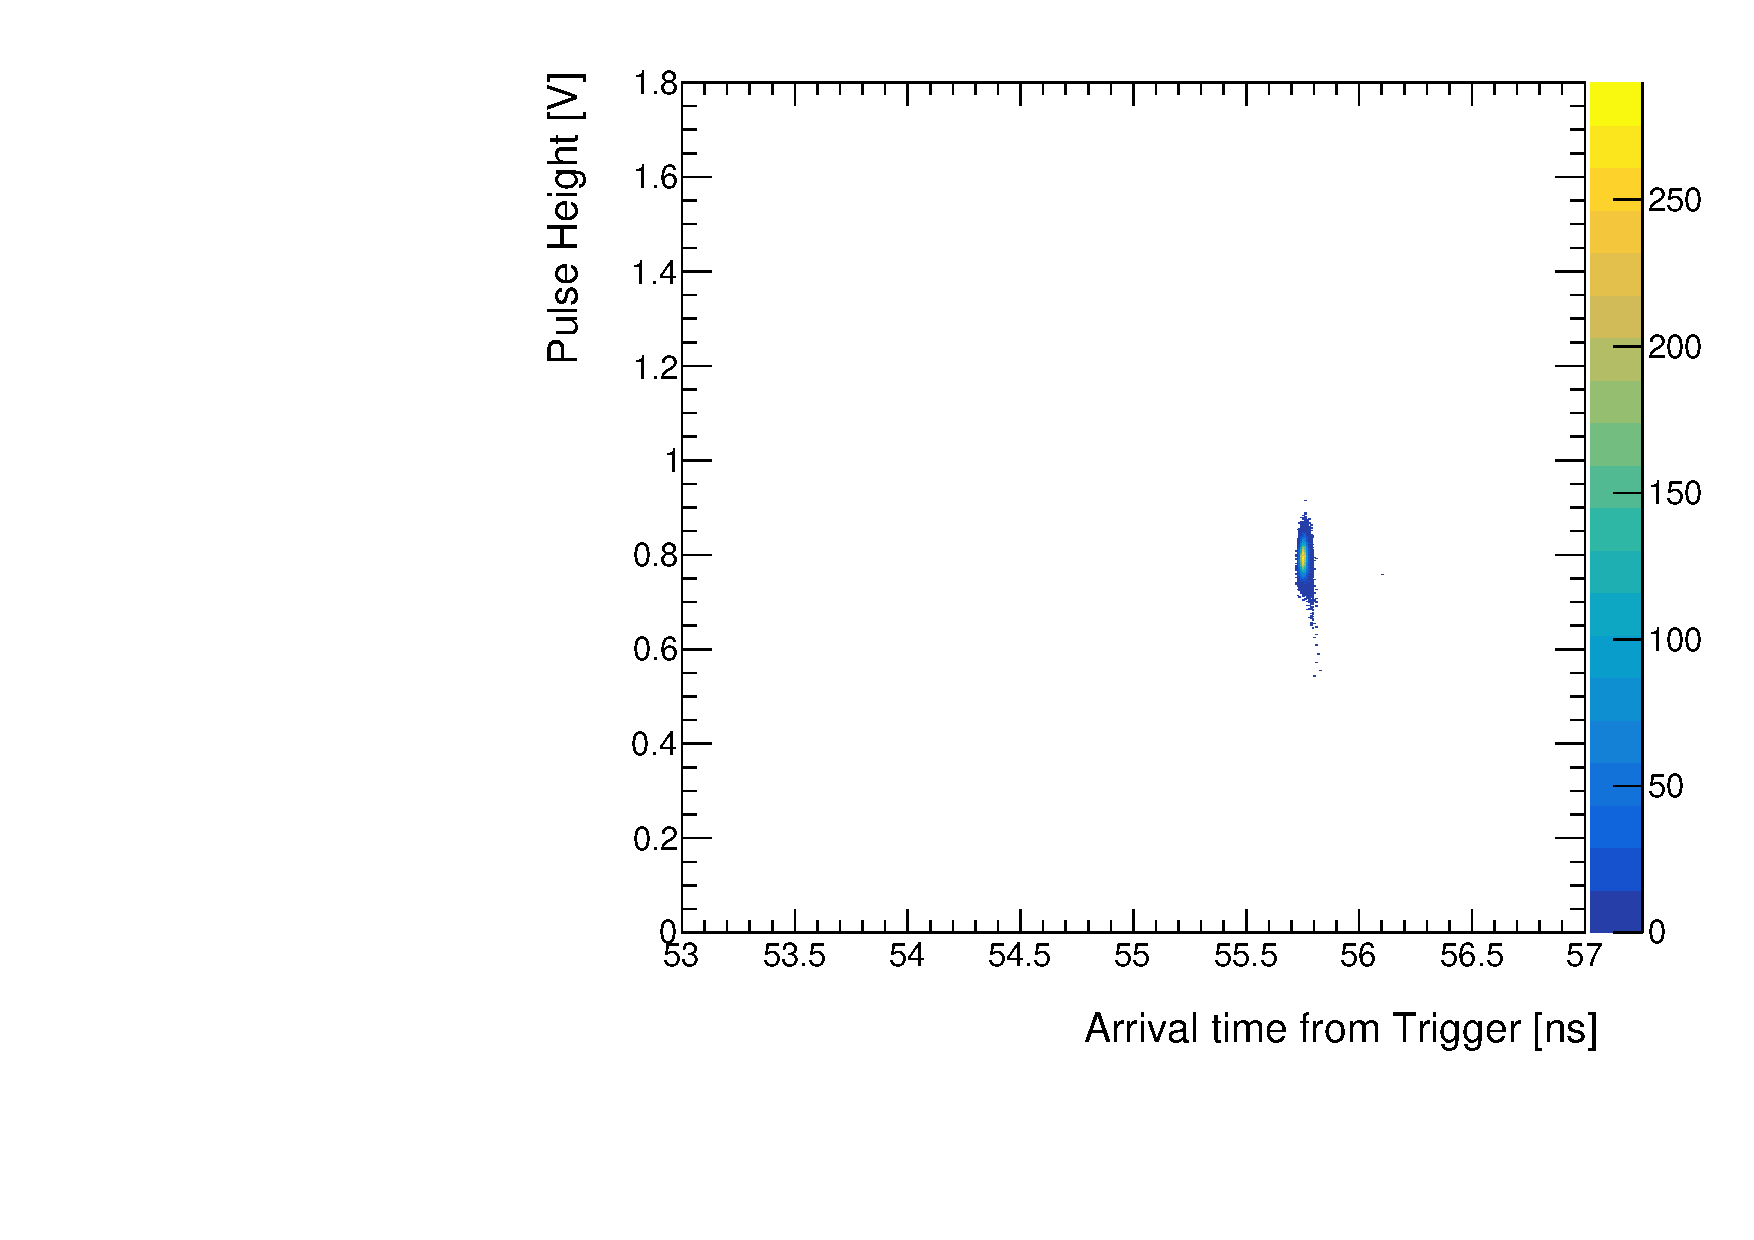
\includegraphics[width=8cm]{fig/graph/phvstime_190V.pdf}
%        \subcaption{190Vの2次元ヒストグラム}
%        \label{fg:APD_2Dhist_190V}
%    \end{minipage}
%    \begin{minipage}[b]{0.5\linewidth}
%        \centering
%        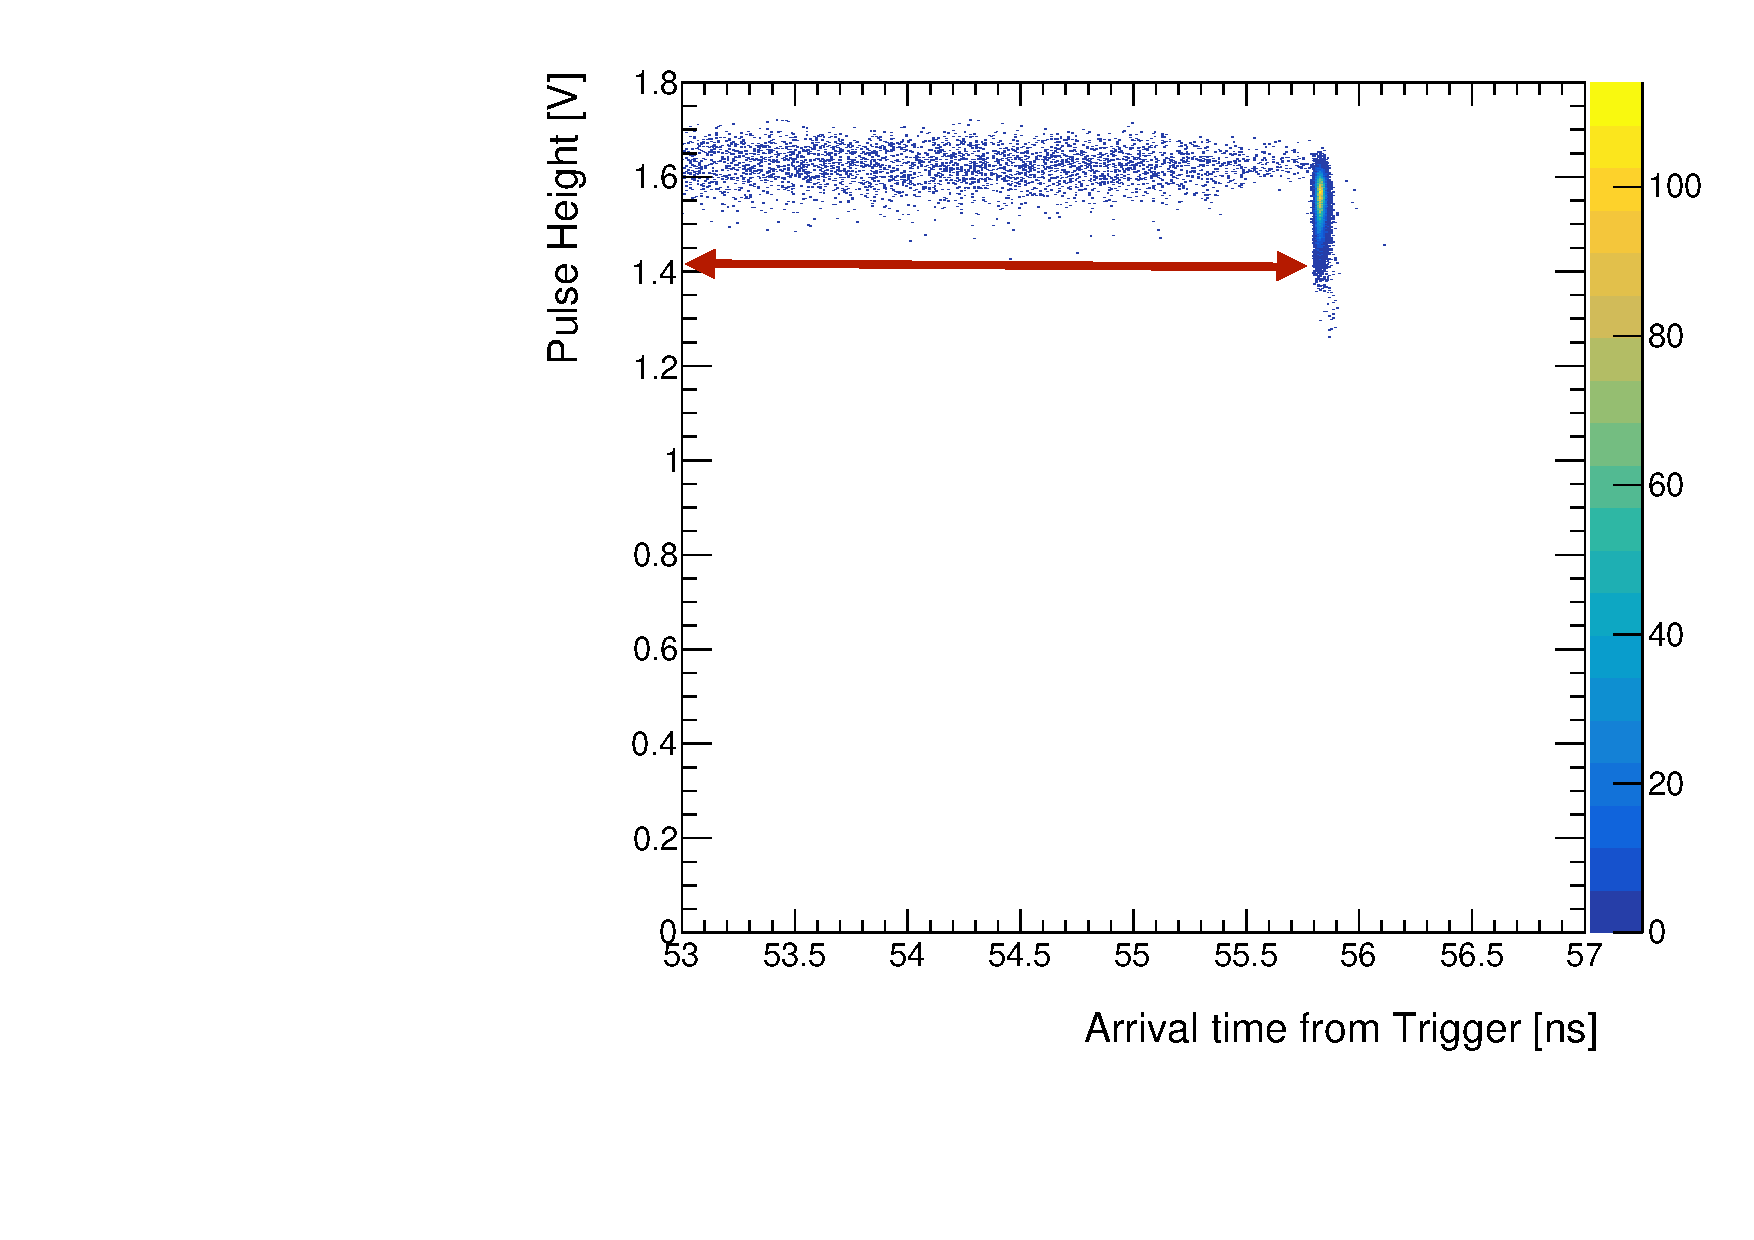
\includegraphics[width=8cm]{fig/graph/phvstime_198V.pdf}
%        \subcaption{198Vの2次元ヒストグラム}
%        \label{fg:APD_2Dhist_198V}
%    \end{minipage}
%    \caption[190Vと198Vの時の到達時間と波高の2次元ヒストグラム]{190Vと198Vの時の到達時間と波高の2次元ヒストグラム\\横軸が到達時間で縦軸が波高、198Vのヒストグラムには波高の変化による到達時間のばらつきが生じている}
%    \label{fg:APD_2Dhist}
%\end{figure}
%
%信号由来の波高のばらつきが到達時間にどのくらい影響を与えるのかを評価するために、波高の50%の標準偏差を$\sigma_s$として、
%以下の 式\ref{eq:sigma_m} のように時間分解能への影響を定義した。
%増幅率が増加すると、信号由来の波高のばらつきの効果が大きくなるため、この影響を$\sigma_{ph}$として議論を進めていく。
%この式の分子に関しては、信号由来の波高の50%の揺らぎ$\sigma_s$からノイズ$\sigma_n$の影響を除いたものとなっている。
%それを信号の傾きで割ることによって、x成分である到達時間の揺らぎ$\sigma_{ph}$を求めることで、信号由来の波高のばらつきによる効果を考えてみる。
%傾きは、ジッター$\sigma_j$の際に計算した、波高の60%から40%間の立ち上がり時間と波高差を用いて求めたものを使用する。
%
%\begin{equation}
%    \sigma_{ph} = \frac{\sqrt{{\sigma_s}^2-{\sigma_n}^2}}{\left|\frac{dV}{dt}\right|} = \frac{\sqrt{{\sigma_s}^2-{\sigma_n}^2}}{\left|\frac{S}{t_r}\right|}
%    \label{eq:sigma_m}
%\end{equation}
%
%
%\subsection{結果}
%以下の 図\ref{fg:/Multiplication_NoisevsVoltage} に、波高の揺らぎによる効果$\sigma_{ph}$の電圧依存性を示す。
%横軸が電圧で縦軸が波高の揺らぎによる効果である。緑点がAPDの計算結果を示している。
%また、PINに関しては、測定したすべての電圧で、波高の50%の揺らぎ$\sigma_s$よりもノイズ$\sigma_n$の方が大きかったため、過剰ノイズの効果は評価できなかった。
%これは、PINの検出器は増幅層がないため、信号の増幅による波高の揺らぎの影響がないからであると考える。
%
%APDの波高の揺らぎの効果は180 V を超えると現れ、電圧上昇によって徐々に上昇していることがわかる。
%今回 式\ref{eq:sigma_m} で求めた時間分解能を増加させる効果は、図\ref{fg:Treso_jitter_MultiplicationvsGain} を見ると、
%増幅率に比例して増加していることがわかった。
%%この180 V 以上で見られる、信号由来の波高のばらつきの増加が、LGAD検出器の時間分解能を悪くする要因であり、
%%それは過剰ノイズの効果であると評価することができた。
%
%
%\begin{figure}[h]
%    \centering
%    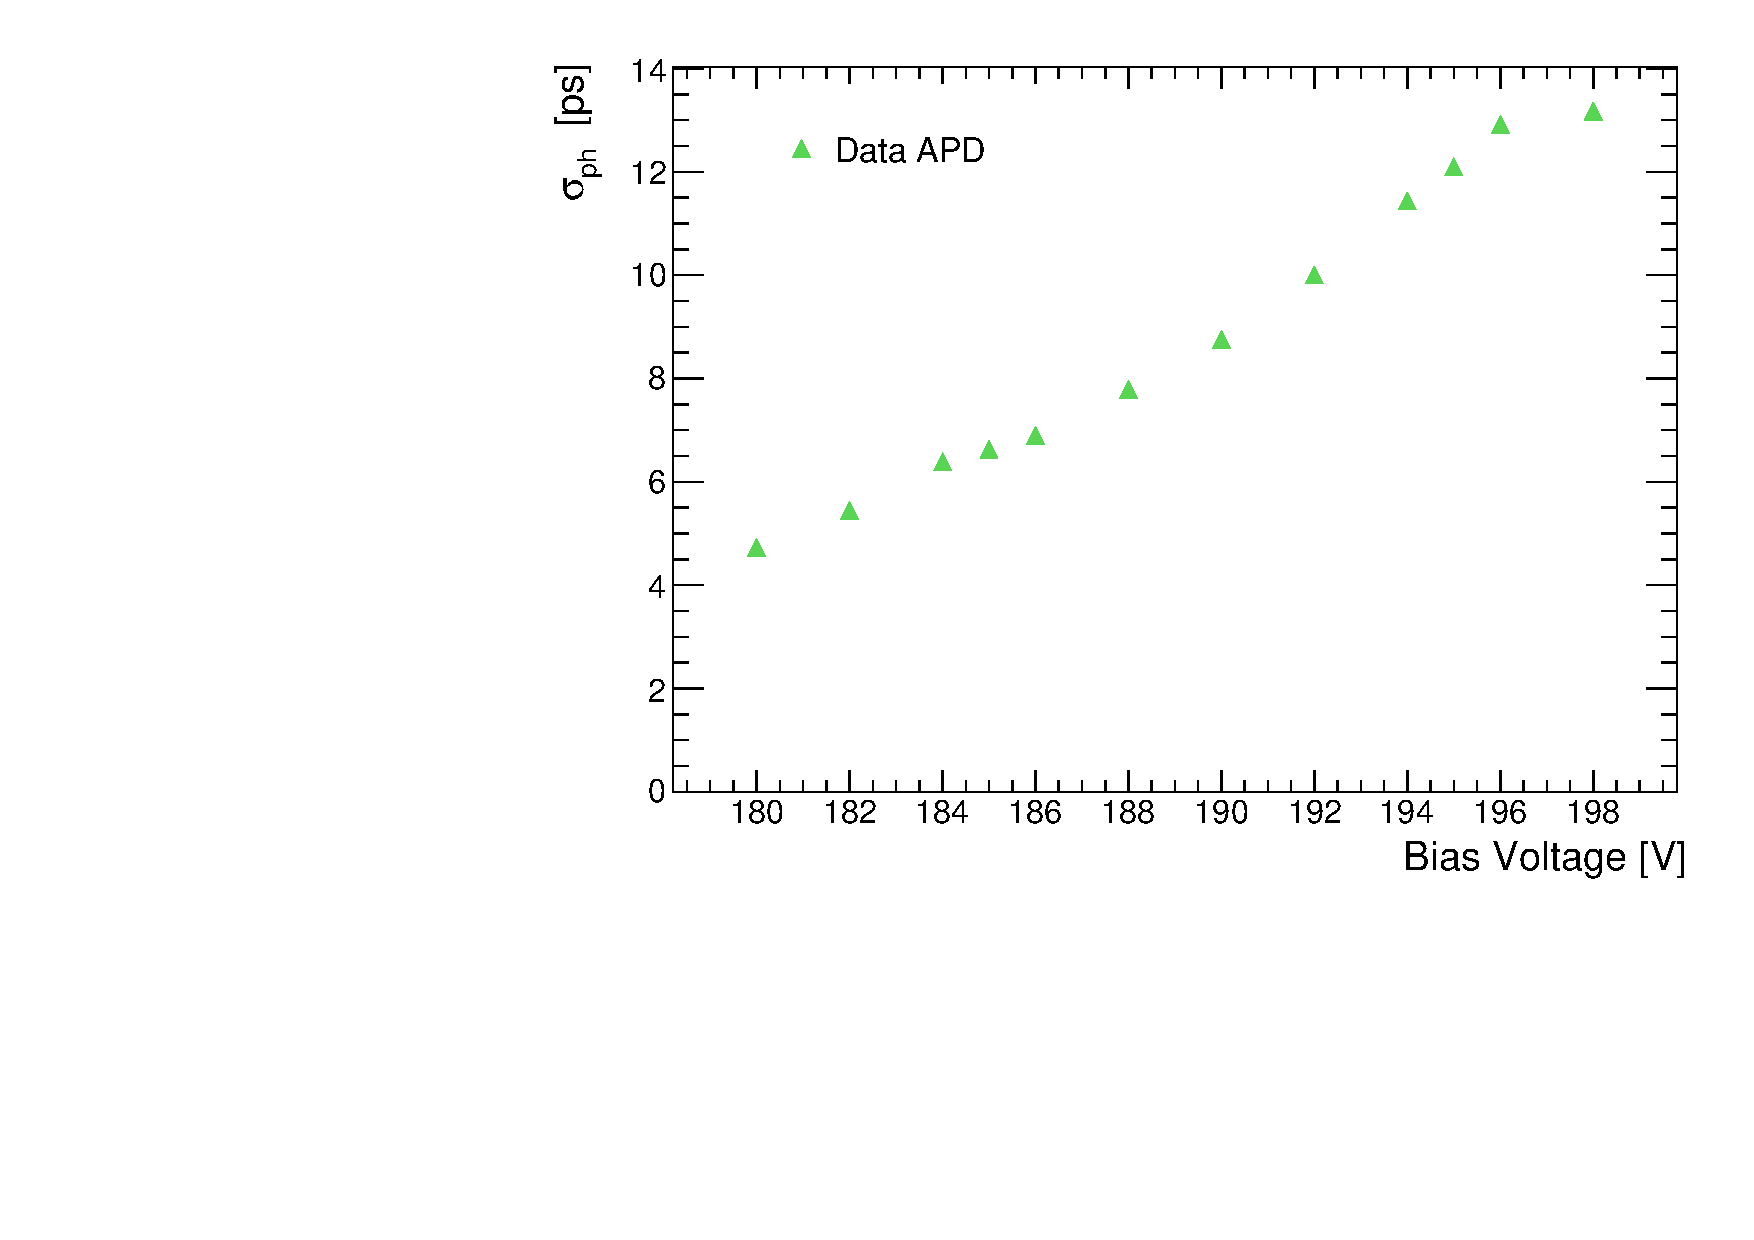
\includegraphics[width=12cm]{fig/graph/Sigma_phvsVoltage.pdf}
%    \caption[AC-LGAD検出器の過剰ノイズの電圧依存性]{AC-LGAD検出器の過剰ノイズの電圧依存性\\横軸が電圧で縦軸が過剰ノイズの効果、緑点がAPDのデータ点}
%    \label{fg:/Multiplication_NoisevsVoltage}
%\end{figure}
%
%これまでに測定した時間分解能$\sigma_t$と、測定値から求めたジッター$\sigma_j$と波高の揺らぎ$\sigma_{ph}$の増幅率依存性を 図\ref{fg:Treso_jitter_MultiplicationvsGain} に示す。
%横軸が増幅率で、縦軸が時間分解能、ジッター、波高の揺らぎによる効果である。青点が時間分解能、赤点がジッター、緑点が波高の揺らぎによる効果を表している。
%このグラフを見ると、ジッター$\sigma_j$は、電圧を上げるほど信号の増幅率が大きくなるため、減少していることがわかる。
%それに対して、波高の揺らぎによる効果$\sigma_{ph}$は、180Vを超えると増加していることがわかる。
%LGAD検出器の時間分解能$\sigma_t$が上昇してしまう原因は、波高の揺らぎによる効果の影響がジッターよりも大きくなるからであると考える。
%
%\begin{figure}[h]
%    \centering
%    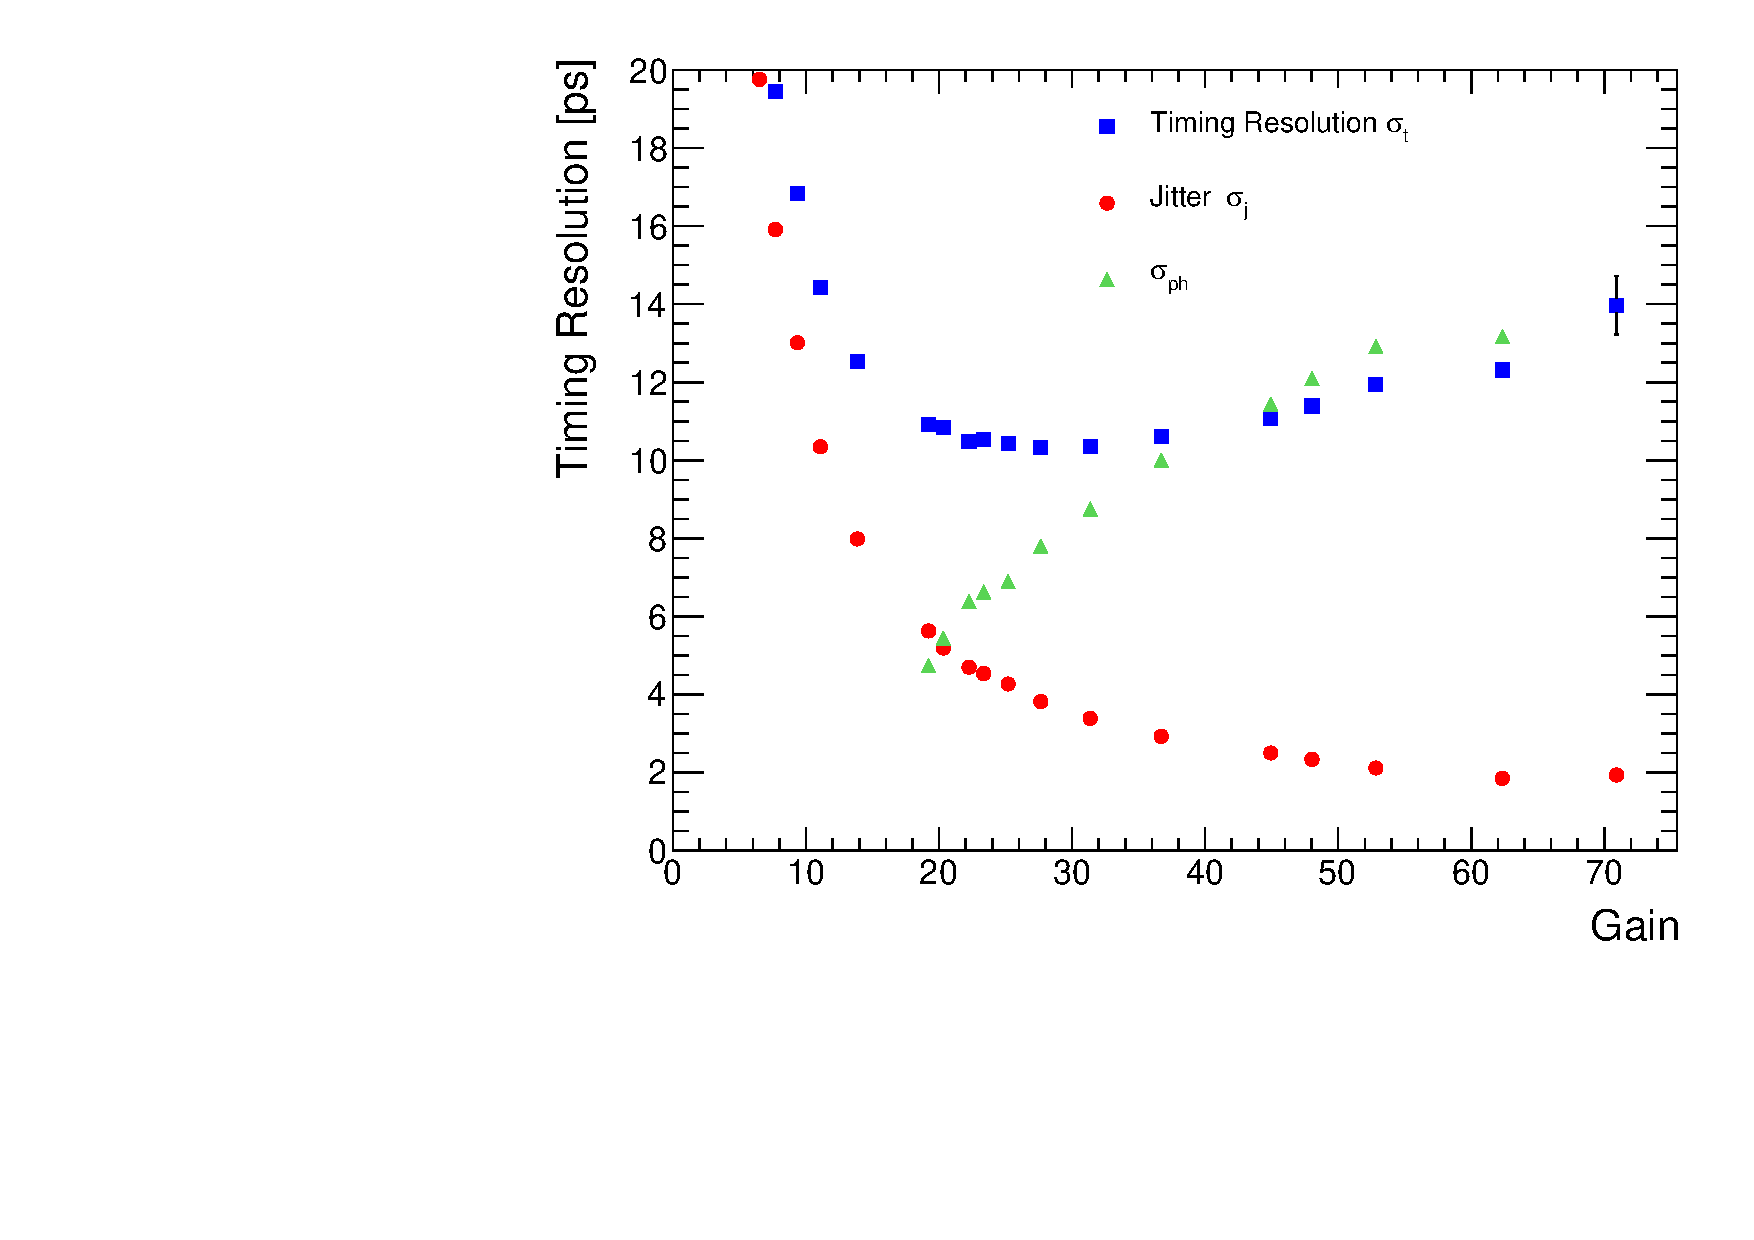
\includegraphics[width=12cm]{fig/graph/Multiplication_Jitter_TresovsGain_0-20ps.pdf}
%    \caption[AC-LGAD検出器のの時間分解能、ジッター、波高の揺らぎによる効果の増幅率依存性]{AC-LGAD検出器のの時間分解能、ジッター、波高の揺らぎによる効果の増幅率依存性\\横軸が増幅率、縦軸が時間分解能とジッターと波高の揺らぎによる効果\\青点が時間分解能$\sigma_t$で赤点がジッター$\sigma_j$で緑点が波高の揺らぎによる効果$\sigma_m$のデータ点}
%    \label{fg:Treso_jitter_MultiplicationvsGain}
%\end{figure}


